\originalchapter{作业七}\label{chap:ps07}
本章译自 MIT 18.650, Fall 2016 官方 \href{https://ocw.mit.edu/courses/18-650-statistics-for-applications-fall-2016/resources/problem-set-7/}{Problem Set 7}, 截止时间为 2016 年 10 月 28 日星期五中午 12 点. 官方仅提供题目, 以下解答为独立推导. 第1题保留原件五幅 QQ 图, 图中的横轴对应标准正态理论分位数, 纵轴对应样本次序统计量.

\begin{exercise}\label{ps07:p01}
原作业第1题. 拉普拉斯分布的密度为 $f_\lambda(x)=\lambda e^{-\lambda|x|}/2$, $\lambda>0$, $x\in\R$; 柯西分布的密度为 $g(x)=1/[\pi(1+x^2)]$. 五个独立同分布样本分别来自标准正态分布、区间 $[-\sqrt3,\sqrt3]$ 上的均匀分布、柯西分布、率参数为1的指数分布、参数为 $\sqrt2$ 的拉普拉斯分布. 对这五个样本画出下列正态 QQ 图. 判断每一幅图对应哪个分布. 本题在原件中没有编号子问.
\begin{center}
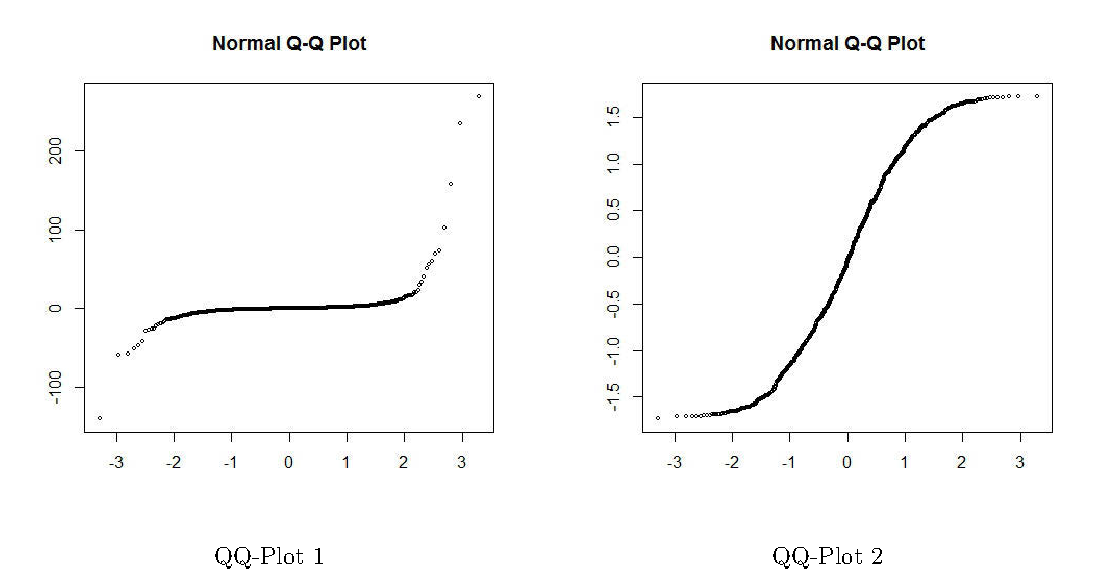
\includegraphics[width=\linewidth]{assignments/assets/ps07-qqplots.pdf}\par
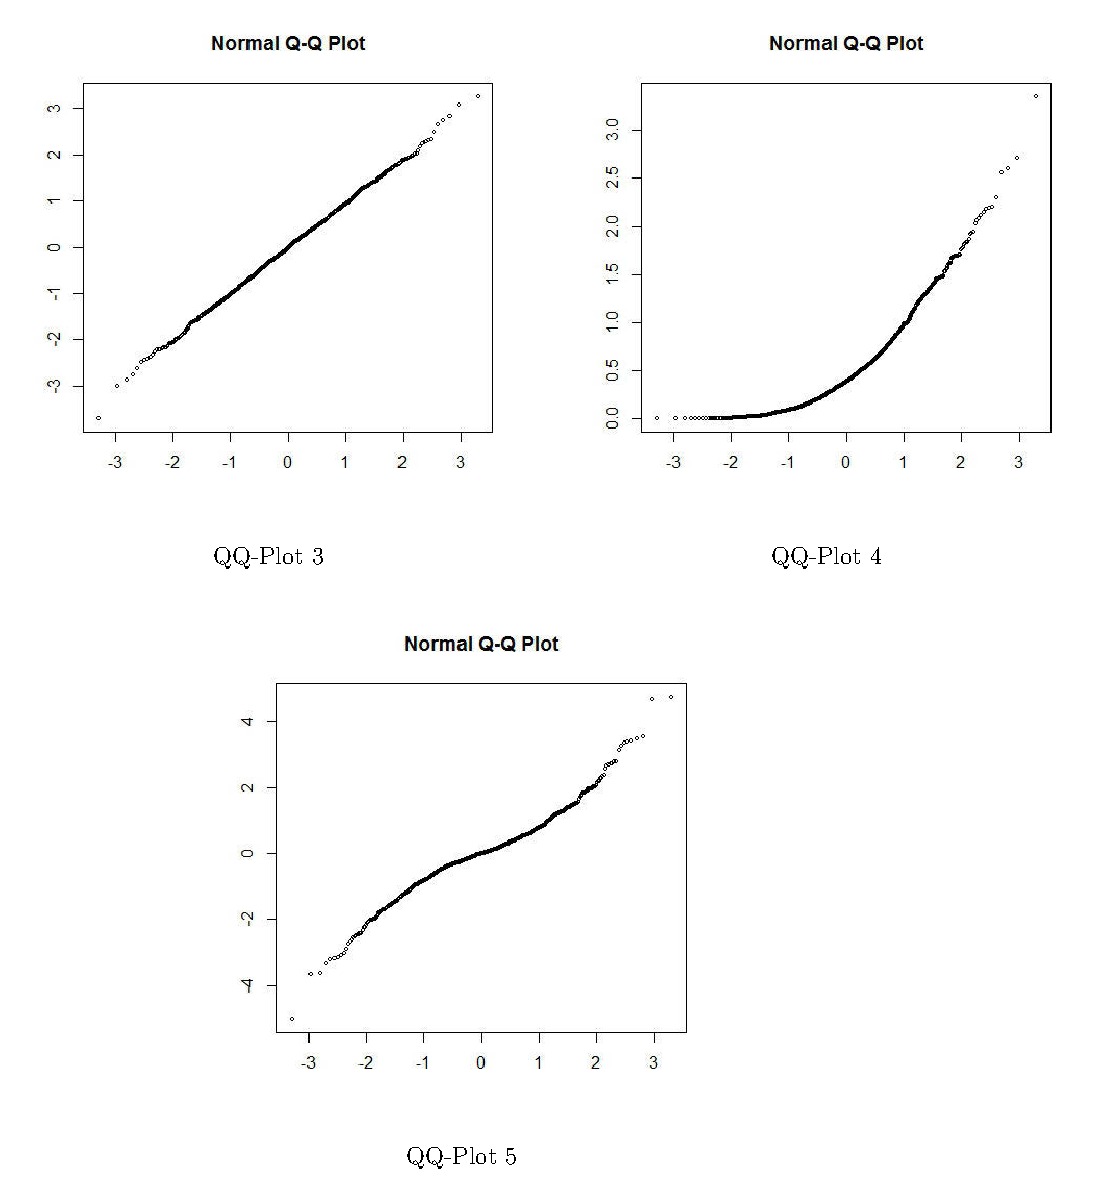
\includegraphics[width=.86\linewidth]{assignments/assets/ps07-qqplots-2.pdf}
\end{center}
\end{exercise}
\begin{solution}
正态 QQ 图将理论正态分位数 $z=\Phi^{-1}(u)$ 与样本经验分位数配对. 总体曲线可用 $F^{-1}(\Phi(z))$ 理解, 样本图围绕该曲线波动. 五图分别是:
\begin{enumerate}[label=图\arabic*:,leftmargin=3em]
\item 柯西分布. 分位数为 $F^{-1}(u)=\tan\{\pi(u-1/2)\}$, 两端发散远快于正态分位数. 图上大部分点挤在零附近, 极端观测达到负百余与正两百余, 是这五个候选中最重的双侧尾.
\item $[-\sqrt3,\sqrt3]$ 上的均匀分布. 总体 QQ 曲线为 $\sqrt3\{2\Phi(z)-1\}$, 近中央斜升, 两端分别趋于 $-\sqrt3$ 与 $\sqrt3$. 图上两端在约 $\pm1.73$ 处变平, 与有界支撑一致.
\item 标准正态分布. 此时 $F^{-1}(\Phi(z))=z$, 因而图形近似斜率1、截距0的直线. 两端有少量抽样波动不改变这一识别.
\item $\operatorname{Exp}(1)$ 分布. 其分位数为 $-\log(1-u)$, 所以总体 QQ 曲线为 $-\log\{1-\Phi(z)\}$. 全部样本非负, 左端贴近0, 右侧向上弯曲并伸出右尾, 图形明显不对称.
\item $\operatorname{Laplace}(\sqrt2)$ 分布. 对 $u<1/2$, 分位数为 $\log(2u)/\sqrt2$; 对 $u\ge1/2$, 为 $-\log\{2(1-u)\}/\sqrt2$. 分布对称且方差为 $2/(\sqrt2)^2=1$, 中央与正态量级接近, 但双侧指数尾比正态尾重. 因而左尾低于直线、右尾高于直线, 尾部偏离比柯西温和, 正是图5.
\end{enumerate}
这些匹配结合了题面限定的五个候选; QQ 图本身不是有限样本下唯一确定分布的证明.
\end{solution}

\begin{exercise}\label{ps07:p02}
原作业第2题. 给定两个独立样本 $X_1,\ldots,X_n$ 与 $Y_1,\ldots,Y_m$, 各样本内部独立同分布, 分布函数分别为 $F,G$. 样本量可不相等. 为简化, 假定两个分布函数连续且递增. 要检验 $H_0:F=G$ 与 $H_1:F\ne G$.
\begin{enumerate}[label=\arabic*.]
\item 给出一个需要判断两个样本是否来自同一分布的实验例子.
\item 令 $U_i=F(X_i)$, $V_j=G(Y_j)$. 求它们的分布.
\item 令 $F_n,G_m$ 为两个样本的经验分布函数.
\begin{enumerate}[label=\alph*)]
\item 定义 $T_{n,m}=\sup_{t\in\R}|F_n(t)-G_m(t)|$. 证明它等于有限个数的最大值.
\item 在 $H_0$ 下证明
\[
T_{n,m}=\sup_{0\le x\le1}\left|\frac1n\sum_{i=1}^n\ind\{U_i\le x\}-\frac1m\sum_{j=1}^m\ind\{V_j\le x\}\right|.
\]
\item 在 $H_0$ 下求 $U_1,\ldots,U_n,V_1,\ldots,V_m$ 的联合分布.
\item 推出 $T_{n,m}$ 为枢轴统计量, 即其原假设分布不依赖未知的总体分布.
\item 给定 $\alpha\in(0,1)$, 令 $q_\alpha$ 为原假设下 $T_{n,m}$ 的 $(1-\alpha)$ 分位数. 如果找不到适合 $n,m$ 的表, 描述一个可在软件(如R)运行的近似分位数算法.
\item 给出非渐近水平 $\alpha$ 的检验.
\end{enumerate}
\end{enumerate}
\end{exercise}
\begin{solution}
\begin{enumerate}[label=\arabic*.]
\item 可随机抽取旧工艺和新工艺生产的电池, 比较其寿命分布. 均值相同并不排除早期失效比例或尾部寿命不同, 所以比较整个分布比只比较均值更符合目标. 两组应相互独立, 各自从固定工艺总体随机抽样.
\item 连续分布函数的概率积分变换给出 $U_i,V_j\sim U[0,1]$. 在严格递增的题设下, 对 $u\in(0,1)$,
$\PP(F(X_i)\le u)=\PP(X_i\le F^{-1}(u))=F(F^{-1}(u))=u$.
同一计算用于 $G$. 变换逐个作用于独立变量, 因此仍保持各样本内部以及两组之间的独立性.
\item
\begin{enumerate}[label=\alph*)]
\item 将合并样本的不同观测值排序为 $w_1<\cdots<w_k$, $k\le n+m$. 两个经验分布函数均在这些点跳跃, 在 $[w_l,w_{l+1})$ 上保持常数; 在第一个点之前均为0, 最后一个点之后均为1. 由右连续性,
\[
T_{n,m}=\max_{1\le l\le k}|F_n(w_l)-G_m(w_l)|.
\]
因此可在有限个观测点精确计算上确界, 不需要连续网格搜索.
\item 在 $H_0$ 下, $F=G$ 且单调变换保持次序, 故 $X_i\le t$ 等价于 $U_i\le F(t)$, $Y_j\le t$ 等价于 $V_j\le F(t)$. 连续递增分布函数的值域含 $(0,1)$, 而端点处两个经验函数的差为0. 因此取 $t\in\R$ 的上确界等于取 $x\in[0,1]$ 的上确界, 得到题中恒等式. 连续但非严格递增的分布函数也可用广义逆证明相同分布结论; 本题使用给定的递增条件即可.
\item 所有 $n+m$ 个变量相互独立且服从 $U[0,1]$. 联合分布为 $[0,1]^{n+m}$ 上的乘积均匀分布.
\item 上问右侧是上述独立均匀向量的确定函数, 故其分布只由整数 $n,m$ 决定, 不涉及 $F$. 这就是原假设下的枢轴性, 而不是宣称备择下也与 $F,G$ 无关.
\item 重复 $B$ 次: 生成 $n+m$ 个独立均匀数, 前 $n$ 个归第一组、后 $m$ 个归第二组; 合并排序并沿排序累积两组计数, 计算最大经验分布差. 将模拟得到的 $B$ 个统计量排序, 取第 $\lceil B(1-\alpha)\rceil$ 个作近似分位数. 下面R代码可直接运行, 不要求输入原始样本:
\begin{verbatim}
ks_stat <- function(x, y) {
  ord <- order(c(x, y))
  lab <- c(rep(1, length(x)), rep(0, length(y)))[ord]
  max(abs(cumsum(lab)/length(x) -
          cumsum(1-lab)/length(y)))
}
ks_quantile <- function(n, m, alpha=.05, B=50000) {
  stopifnot(n>=1, m>=1, alpha>0, alpha<1)
  val <- replicate(B, ks_stat(runif(n), runif(m)))
  sort(val)[ceiling(B*(1-alpha))]
}
set.seed(65007)
ks_quantile(20, 25)
\end{verbatim}
$n=20,m=25$ 只是算法验算的示例, 原题没有指定数值. 对 $\alpha=0.05$, Python 等价算法的50000次模拟得到分位数约0.39. 本项目实际运行了 Python 的等价算法, 没有运行R. 模拟分位数有抽样误差, 不能把有限 $B$ 的估计误说成已知的精确临界值.
\item 定义精确分位数 $q_\alpha=\inf\{q:\PP_0(T_{n,m}\le q)\ge1-\alpha\}$. 当 $T_{n,m}>q_\alpha$ 时拒绝, 则 $\PP_0(T_{n,m}>q_\alpha)\le\alpha$. 此统计量的分布是离散的, 一般不能保证不随机化的检验大小恰为 $\alpha$; “水平 $\alpha$”指至多 $\alpha$. 精确分位数可以枚举合并排序中 $\binom{n+m}{n}$ 种等概率组标签次序求得. 模拟近似临界值本身只近似控制水平.

若只用有限次模拟而仍要求严格有限样本控制, 可生成 $B$ 个独立原假设统计量 $T^{(b)}$, 取
$p_{\rm MC}=\{1+\sum_b\ind(T^{(b)}\ge T_{\rm obs})\}/(B+1)$,
在 $p_{\rm MC}\le\alpha$ 时拒绝. 原假设下观察值与模拟值交换对称; 以大于等于计数使并列保守, 所以秩检验的拒绝概率至多 $\alpha$. 这一规则把模拟随机性也计入检验, 避免将估计分位数当作精确分位数.
\end{enumerate}
\end{enumerate}
\end{solution}

\begin{exercise}\label{ps07:p03}
原作业第3题. 给定独立同分布实随机变量对 $(X_i,Y_i)$, $i=1,\ldots,n$, 其分布连续. 要检验 $H_0:X_1,Y_1\text{ 独立}$ 与 $H_1:X_1,Y_1\text{ 不独立}$. 令 $R_i$ 为 $X_i$ 在 $X_1,\ldots,X_n$ 中的秩, 最小值秩为1, 最大值秩为 $n$; $Q_i$ 为 $Y_i$ 的相应秩.
\begin{enumerate}[label=\arabic*.]
\item 给出需要检验两组观测独立性的实验例子.
\item 不必严格证明, 解释为什么 $R_1,\ldots,R_n$ 不独立.
\item 证明 $R$ 的分布不依赖 $X_i$ 的未知分布, $Q$ 的分布也不依赖 $Y_i$ 的未知分布.
\item 证明在 $H_0$ 下, 两个秩向量 $R,Q$ 相互独立.
\item 推出在 $H_0$ 下, 所有 $2n$ 个秩的联合分布已知且不依赖原样本分布.
\item 定义秩的样本相关系数
\[
T_n=\frac{\sum_i(R_i-\bar R)(Q_i-\bar Q)}{\sqrt{\sum_i(R_i-\bar R)^2\sum_i(Q_i-\bar Q)^2}}.
\]
\begin{enumerate}[label=\alph*)]
\item 证明 $\bar R=\bar Q=(n+1)/2$, $\sum_i(R_i-\bar R)^2=\sum_i(Q_i-\bar Q)^2=n(n^2-1)/12$. 提示: $\sum_{i=1}^ni=n(n+1)/2$, $\sum_{i=1}^ni^2=n(n+1)(2n+1)/6$.
\item 推出 $T_n=12\sum_iR_iQ_i/[n(n^2-1)]-3(n+1)/(n-1)$.
\end{enumerate}
\item 证明在 $H_0$ 下 $T_n$ 与
$S_n=12\sum_iR'_iQ'_i/[n(n^2-1)]-3(n+1)/(n-1)$ 同分布, 其中 $R',Q'$ 来自两组相互独立的独立同分布 $U[0,1]$ 样本.
\item 给定 $\alpha\in(0,1)$, 令 $q_\alpha$ 为 $S_n$ 的 $(1-\alpha)$ 分位数. 描述给定 $n$ 时可在R中近似计算它的算法.
\item 定义 $H_0$ 对 $H_1$ 的非渐近水平 $\alpha$ 检验.
\end{enumerate}
\end{exercise}
\begin{solution}
秩相关要求 $n\ge2$ 且各边际无原子, 于是各组内部几乎处处没有并列值. 这里“连续分布”按无并列所需的边际连续解释; 不额外假定联合密度存在. 若只要求二维分布没有点原子, 却容许边际原子, 原题的无并列秩结论就需另补条件.
\begin{enumerate}[label=\arabic*.]
\item 可以对随机抽取的同一批成年人的每日运动时长与静息心率作成对测量, 检验两者是否独立. 每人的两项观测保持配对, 不同受试者独立抽样.
\item 每个秩只可出现一次. 如果 $R_1=n$, 其余秩都不能再等于 $n$; 知道前 $n-1$ 个秩后, 最后一个秩已被确定. 因此秩之间相互约束, 不是独立变量.
\item 对任意排列 $\pi$, 事件 $X_{\pi(1)}<\cdots<X_{\pi(n)}$ 具有相同概率: 独立同分布使联合分布在任意指标置换下不变. 无并列使这 $n!$ 个事件互斥且覆盖概率1, 所以每个事件概率为 $1/n!$. 每个事件唯一对应一个秩向量, 因而 $R$ 在所有 $\{1,\ldots,n\}$ 的排列上均匀分布. 证明不使用边际分布具体形式. 对 $Q$ 完全相同.
\item 成对样本的联合分布为 $\prod_iP_{XY}$; 在 $H_0$ 下 $P_{XY}=P_X\otimes P_Y$, 所以它重新分组为 $\prod_iP_X\otimes\prod_iP_Y$. 因而整个 $X$ 样本向量与整个 $Y$ 样本向量独立. 可测函数保持独立性, $R=R(X)$ 与 $Q=Q(Y)$ 故独立.
\item 联合秩分布是在 $n!\times n!$ 个排列对上的均匀分布, 每对概率 $1/(n!)^2$. 同一向量内部的秩仍有依赖, 只有两个向量相互独立.
\item
\begin{enumerate}[label=\alph*)]
\item 秩向量只是 $1,\ldots,n$ 的置换, 因而平均为 $(n+1)/2$. 记 $c=(n+1)/2$, 利用题给求和式,
\begin{align*}
\sum_i(R_i-c)^2
&=\frac{n(n+1)(2n+1)}6-2c\frac{n(n+1)}2+nc^2\\
&=n(n+1)\left\{\frac{2n+1}6-\frac{n+1}2+\frac{n+1}4\right\}
=\frac{n(n^2-1)}{12}.
\end{align*}
对 $Q$ 的计算相同, 所以分母是这个确定的正常数.
\item 展开分子, 利用 $\sum_iR_i=\sum_iQ_i=nc$, 得
$\sum_i(R_i-c)(Q_i-c)=\sum_iR_iQ_i-nc^2$.
除以 $n(n^2-1)/12$, 得
\[
T_n=\frac{12}{n(n^2-1)}\sum_iR_iQ_i-
\frac{12nc^2}{n(n^2-1)}
=\frac{12}{n(n^2-1)}\sum_iR_iQ_i-\frac{3(n+1)}{n-1}.
\]
\end{enumerate}
\item 两组独立均匀样本的秩恰有第5问的已知联合分布. 将同一确定函数作用于同分布的 $(R,Q)$ 与 $(R',Q')$, 得 $T_n\stackrel{\mathrm d}=S_n$.
\item 可以逐次产生两组长度 $n$ 的均匀样本, 各自求秩后代入第7问公式; 将 $B$ 个值排序取第 $\lceil B(1-\alpha)\rceil$ 个. 更快的等价算法是在每次模拟生成两个独立均匀随机排列. 由共同指标重排, 还可以固定第一个秩向量为 $1,\ldots,n$, 仅随机生成第二个排列. 下面代码同时给出题面单侧分位数和下一问需要的双侧分位数:
\begin{verbatim}
spearman_quantiles <- function(n, alpha=.05, B=50000) {
  stopifnot(n>=2, alpha>0, alpha<1)
  r <- seq_len(n) - (n+1)/2
  den <- sum(r*r)
  val <- replicate(B, sum(r*(sample.int(n)-(n+1)/2))/den)
  k <- ceiling(B*(1-alpha))
  c(one_sided=sort(val)[k], two_sided=sort(abs(val))[k])
}
set.seed(65007)
spearman_quantiles(10)
\end{verbatim}
本项目运行的是对应 Python 算法, 未运行R. 在 $n=10$, $\alpha=0.05$ 的50000次模拟示例中, 单侧分位数约0.55152, 绝对值分位数约0.63636. 精确分布可在规模允许时枚举 $n!$ 个排列而得. $n=10$ 为验算示例, 不属于原题给定数据.
\item 按原题第8问的单侧 $q_\alpha$, 拒绝规则 $T_n>q_\alpha$ 满足 $\PP_0(T_n>q_\alpha)\le\alpha$, 所以确为非渐近水平 $\alpha$ 的检验. 但原题备择是一般“不独立”, 单侧规则只寻找正秩关联. 例如 $X\sim U[0,1]$, $Y=1-X$, 两者有连续边际且完全相依, 样本秩反序, $T_n=-1$, 该上尾规则无法识别它.

适合正负秩关联的数学版本应令 $c_\alpha$ 为 $|S_n|$ 的 $(1-\alpha)$ 分位数, 在 $|T_n|>c_\alpha$ 时拒绝. 枢轴性给出 $\PP_0(|T_n|>c_\alpha)\le\alpha$. 原题单侧分位数不被暗改成双侧分位数, 二者定义与用途不同. 两种精确规则因离散分布均可能保守; 有限模拟时可沿用上一题的加一 Monte Carlo $p$ 值, 把统计量改成 $|T|$ 以保持双侧水平控制.

即使使用双侧秩相关检验, 也不能声称对所有不独立备择一致. 例如 $X\sim U[-1,1]$, $Y=X^2$, 明显相依, 两边际均连续. 总体秩相关为 $\operatorname{Corr}((X+1)/2,|X|)=0$, 因为 $\E[X|X|]=0$. 此检验针对秩相关偏离零, 不能完全代替一般独立性检验.
\end{enumerate}
\end{solution}
